\documentclass[12pt]{article}

% format
% \usepackage[a4paper, total={6in, 9in}]{geometry}                         

% math symbols
\usepackage{amsmath}
\usepackage{amsthm}
\usepackage{amssymb}
\usepackage[shortlabels]{enumitem} 
\usepackage{mathtools}
\usepackage{bbm}

% annotations
\setlength{\marginparwidth}{2cm}
\usepackage{soul}
\usepackage{pdfcomment}

% figures
\usepackage{graphicx}
\usepackage{subcaption}

% theorems
\theoremstyle{definition}
\newtheorem{thm}{Theorem}
\newtheorem{prop}[thm]{Proposition}
\newtheorem{lemma}[thm]{Lemma}
\newtheorem{rmk}[thm]{Remark}
\newtheorem{defn}[thm]{Definition}
\newtheorem{cor}[thm]{Corollary}
\newtheorem{exo}[thm]{Exercise}
\newtheorem{fact}[thm]{Fact}
\newtheorem{obs}[thm]{Observation}

% definition equal
\newcommand{\defeq}{\vcentcolon=}
\newcommand{\eqdef}{=\vcentcolon}
\pdfcommentsetup{color=yellow, opacity=0.5}

% bibliography
\usepackage[backend=biber,style=alphabetic, sorting=ynt]{biblatex}
\bibliography{ref}

% url highlight
\usepackage{hyperref}

% algos
\usepackage[linesnumbered,ruled,vlined]{algorithm2e}
\SetArgSty{textnormal}

% bullet point style
% \renewcommand{\labelitemi}{\tiny$\blacksquare$}

% new commands
\DeclareMathOperator{\dom}{dom}
\DeclareMathOperator{\Hess}{\textbf{H}}
\DeclareMathOperator{\Diag}{Diag}
\DeclareMathOperator{\Tr}{Tr}
\DeclareMathOperator{\ind}{i}
\DeclareMathOperator{\sgn}{sign}

% figures
\usepackage{tikz}
\usepackage{caption}

% colors
\definecolor{azure}{RGB}{41, 50, 65}
\definecolor{orange}{RGB}{238, 108, 77}
\definecolor{lightblue}{RGB}{224, 251, 252}
\definecolor{blue}{RGB}{152, 193, 217}
\definecolor{darkblue}{RGB}{61, 90, 128}
\definecolor{green}{RGB}{67, 170, 139}
\definecolor{purple}{RGB}{199, 125, 255}

\begin{document}
    
    This work has as its starting
    point the following paper \cite{kchord_ori}.

    \section{Finding induced \texorpdfstring{$k$}{k}-chords in half graphs}
    
    The aim of this section 
    is to prove the following 
    proposition.

    \begin{prop} \label{prop:hg}
        For any $k \neq 1, 4$,
        there exists $n \in \mathbb{N}$
        such that the half
        graph $H_{n}$ 
        contains an induced 
        $k$-chord.
    \end{prop}

    Before tackling the
    above statement, we notice the
    following fact.
    
    \begin{fact} \label{fact:edges}
        For any graph $G$
        and cycle $C$ in $G$, 
        the number of chords in $C$ 
        is given by $e\left(G\left[V\left(C\right)\right]\right)
        - \left|C\right|$.
    \end{fact}
    
    We now establish 
    some notation. For
    any half graph $H_{n}$ 
    with $n \geq 3$, label
    its vertices as follows.
    \begin{figure}[ht]
        \centering
        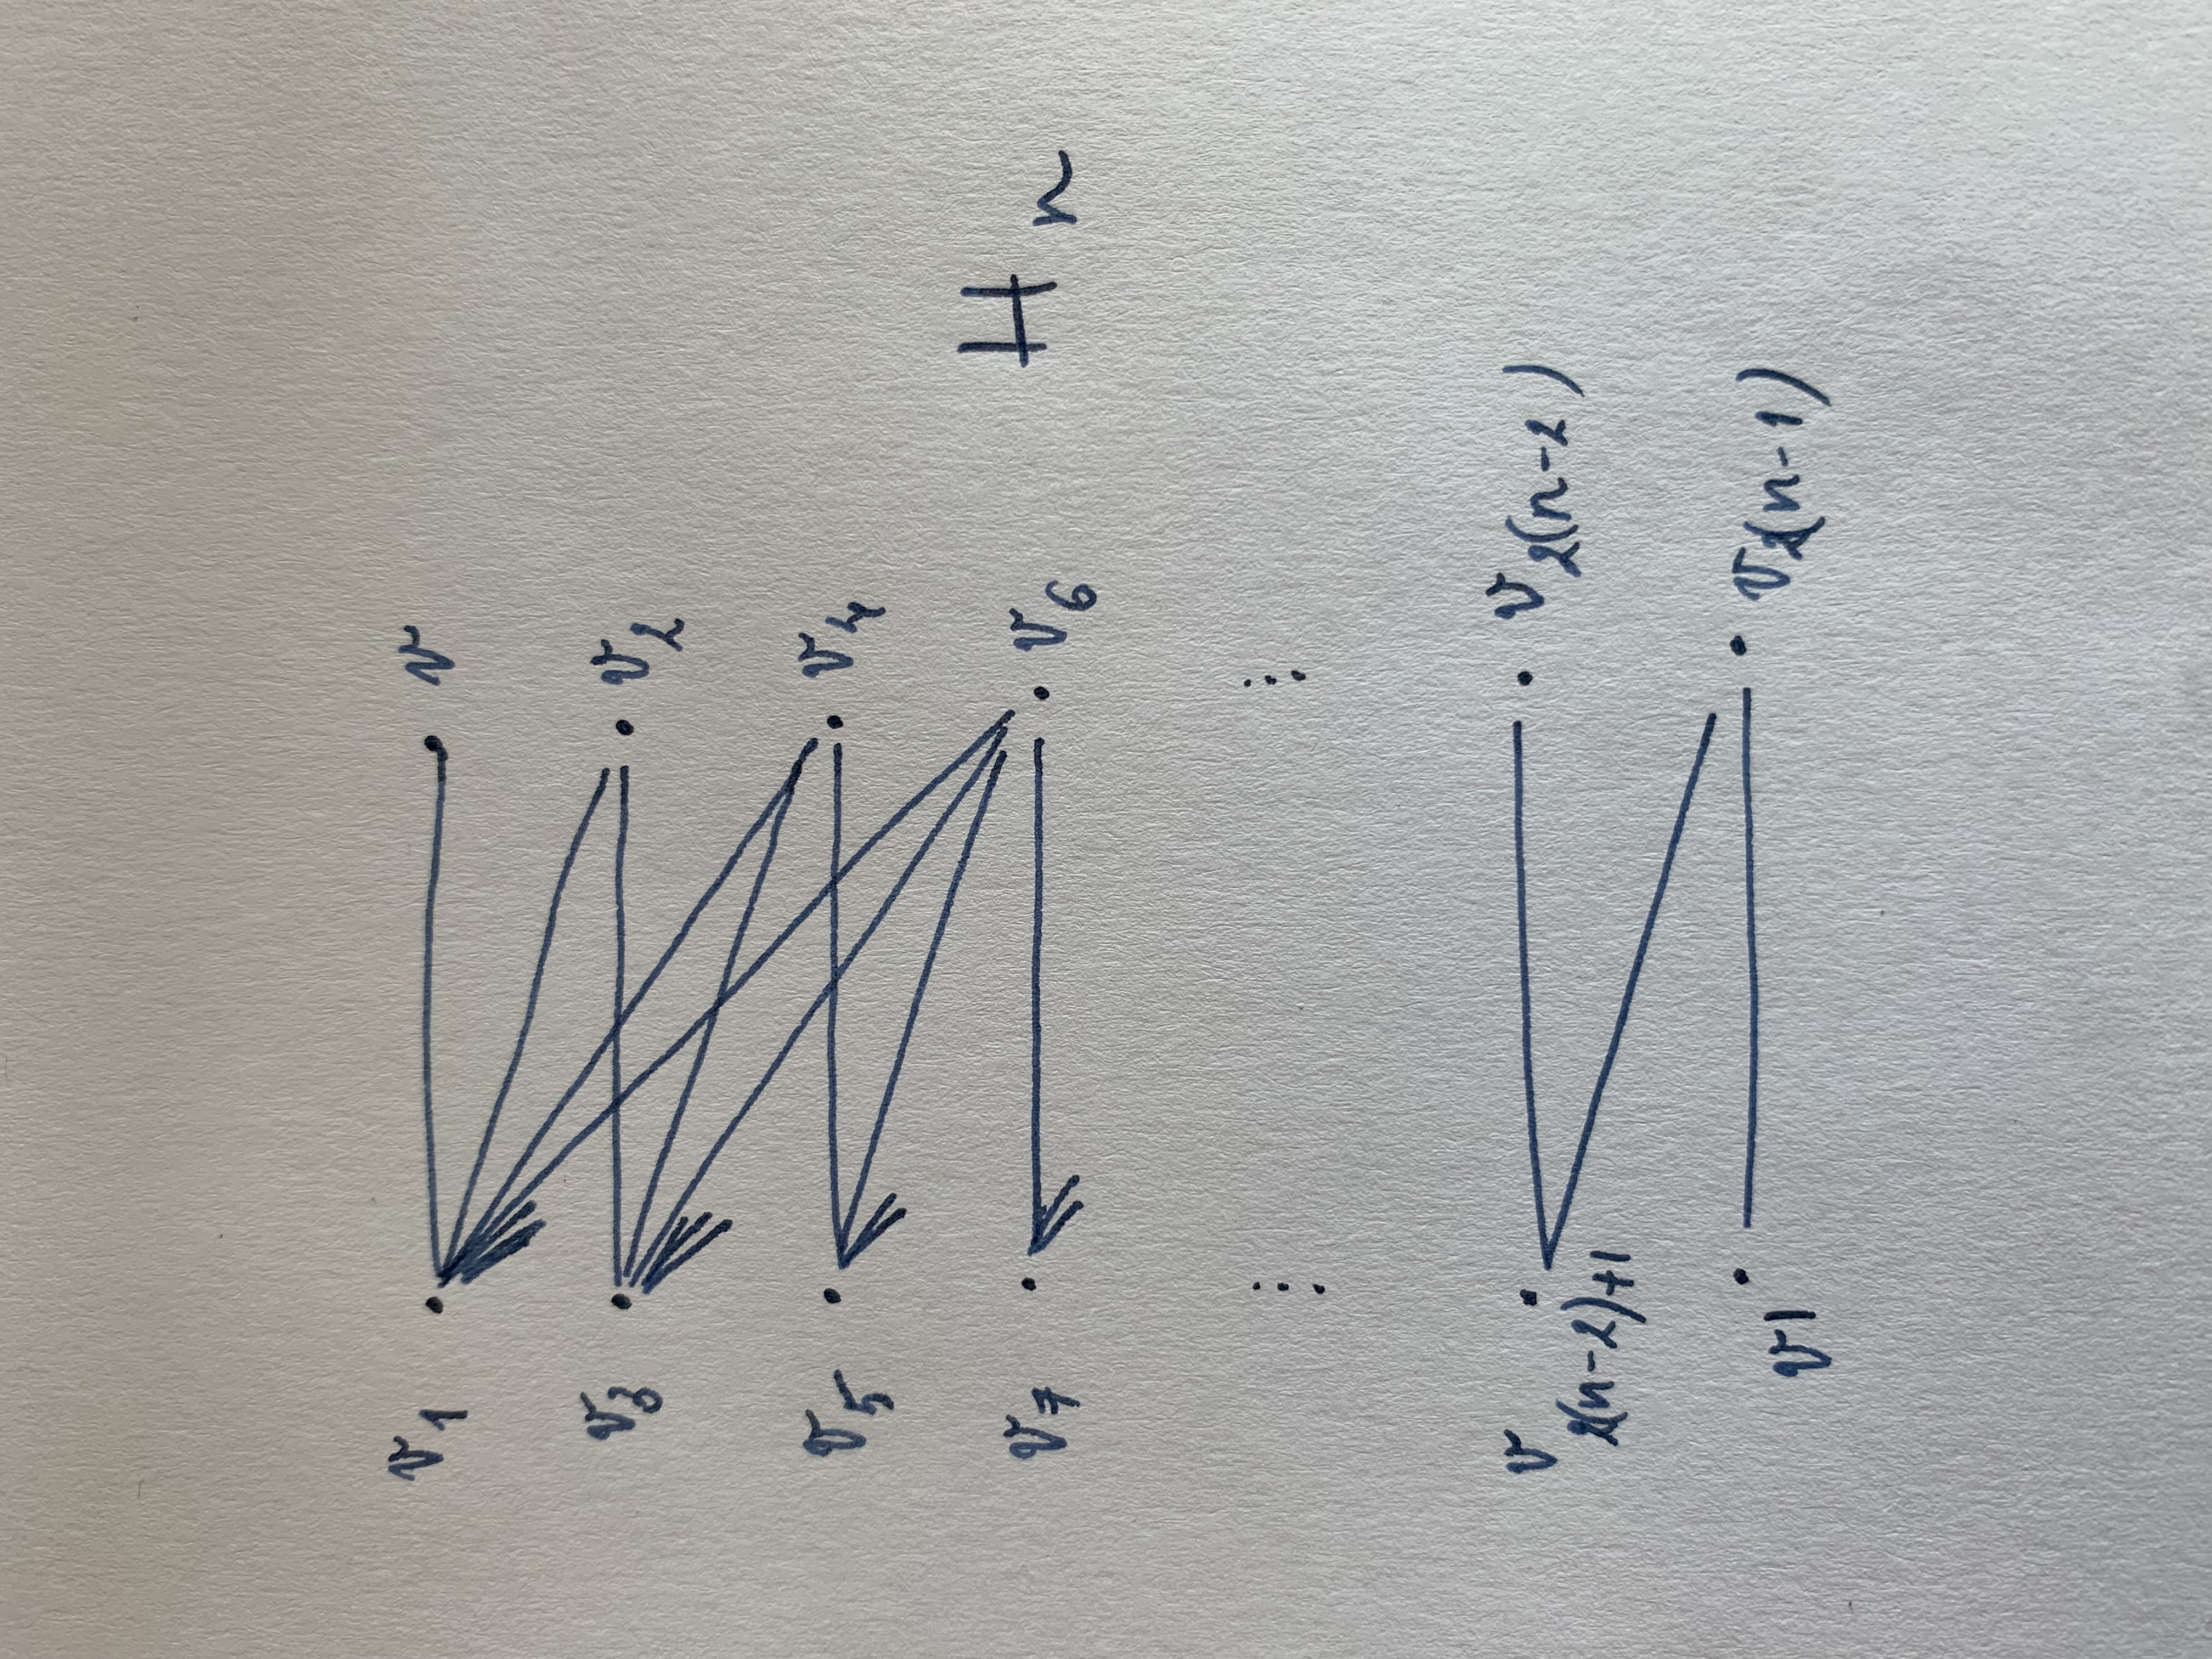
\includegraphics[width=0.5\linewidth, angle=270]{figures/hgraph.jpg}
        \caption{Vertex labeling of a half graph}
        \label{fig:hg}
    \end{figure}

    Notice that the cycle
    $\left(v_1, v_2, \ldots,
    v_{2\left(n-1\right)}, v_1\right)$ 
    induces a $k$-chord
    $C_{n}$ in $H_{n}$
    with the number $K_{n}$ 
    of chords being (by Fact \ref{fact:edges}):
    \begin{gather*}
        K_{n} = \left(
        2 + 3 + \cdots + \left(n-1\right)
        + \left(n-1\right)\right)
        -2\left(n-1\right) =
        \frac{n\left(n-3\right)}{2}.
    \end{gather*}
    
    We now notice the following fact
    which will be useful in the next proofs.

    \begin{fact} \label{fact:new}
        Given a $K_{n}$-chord 
        $C_{n}$, one can obtain
        a new $k$-chord by removing
        vertices $v_{2n_1}, 
        v_{2n_2}, \ldots,
        v_{2n_{m}}, v_{2n_1'+1}, 
        v_{2n_2'+1}, \ldots,
        v_{2n_{m}' + 1}$
        such that
        $n_1 < n_2 < \cdots
        < n_{m} < n_1' < n_2'
        < \ldots, n_{m}'$.
        This last condition is
        necessary to ensure that 
        the vertices in $V\left(C_{n}\right)
        \setminus \left\{
        v_{2n_1}, \ldots, 
        v_{2n_{m}},
        v_{2n_1'+1}, \ldots,
        v_{2n_{m}'+1}\right\}$
        are part of a unique cycle.
        The cycle (and the relative
        induced $k$-chord)
        we take into consideration is
        \begin{gather*}
            \left(v_{2i_1 + 1}, 
            v_{2j_1}, \ldots,
            v_{2i_{n-m}+1},
            v_{2j_{n-m}},
            v_{2i_1 + 1}\right),
        \end{gather*}
        where 
        $\left\{i_1, \ldots, i_{n-m}\right\} =
        \left\{1, \ldots, n\right\} \setminus 
        \left\{n_1', \ldots, n_{m}'\right\}$
        and
        $\left\{j_1, \ldots j_{n-m}\right\}
        = \left\{1, \ldots, n\right\}
        \setminus \left\{n_1, \ldots, n_{m}\right\}$ 
        with $i_1 < \cdots < i_{n-m}$
        and
        $j_1 < \cdots < j_{n-m}$.
    \end{fact}
    
    Now, notice that for any
    $n \geq 4$, we have that
    $K_{n} - K_{n-1} = n-2$.
    Our strategy is to find
    and induced $k$-chord
    into $H_{n}$ with
    $K_{n-1} \leq k \leq K_{n}$ 
    for al $k \neq 1,4$.
    The following lemma
    represents a step towards 
    this objective.

    \begin{lemma} \label{lemma:most}
        For any  $n \geq 4$ and
        any $2 \leq l \leq K_{n}-2$,
        we have that $C_{n}$ contains an induced
        $\left(K_{n} - l\right)$-chord
        (and thus, so does $H_{n}$).
    \end{lemma}
    \begin{proof}
        Let $q = l-1$. Notice that
        $C_{n}$ has the following
        cycle, obtained from $C_{n}$
        by removing $v_{2q}$ and
        $v_{2\left(n-2\right)+1}$
        as in Fact \ref{fact:new}.
        We have:
        \begin{gather*}
            C_{n}' \defeq
            \left(v_1, v_2, \ldots,
            v_{2\left(q-1\right)+1},
            v_{2\left(q+1\right)}, \ldots ,
            v_{2\left(n-2\right)},
            v_{2\left(n-3\right) + 1},
            v_{2\left(n-1\right)}, v_1\right)
        \end{gather*}
        By Fact \ref{fact:new}, 
        $C_{n}'$ induces a $k$-chord
        for some $k$.
        Notice that
        $d\left(v_{2q}\right) = q+1 = l$
        and $d\left(v_{2\left(n-2\right)+1}\right) = 2$.
        Since $\left|C_{n}'\right| = 
        \left|C_{n}\right| - 2$, 
        Fact \ref{fact:edges} tells
        us that the number of 
        induced chords of $C_{n}'$ is
        \begin{gather*}
            K_{n} - \left(l + 2\right) + 2 = K_{n} - l.
        \end{gather*}
        
        This concludes the proof.
    \end{proof}

    Now, notice that $K_{4} = 2$ and $K_{5} = 5$.
    Thus, in order to prove Proposition \ref{prop:hg},
    it suffices to find $n$ such that $H_{n}$ contains
    an induced $\left(K_{m}-1\right)$-chord for
    all $m \geq 6$. We claim that such $n$ is $m+1$.

    \begin{lemma} \label{lemma:remainder}
        For any $m \geq 6$, we have that $C_{m+1}$ contains
        an induced $\left(K_{m} - 1\right)$-chord
        (and thus, so does $H_{m+1}$).
    \end{lemma}
    \begin{proof}
        Consider the $K_{m+1}$-chord $C_{m+1}$.
        Just as in the proof of Lemma \ref{lemma:most},
        consider the $k$-chord $C_{m+1}''$ obtained
        from $C_{m+1}$ by removing the vertices
        $v_2$, $v_{2\left(n-5\right)}$
        $v_{2\left(n-3\right)+1}$, $v_{2\left(n-2\right)+1}$.
        The cycle of $C_{m+1}''$ that
        we will consider is the one
        described in Fact \ref{fact:new}.
        Notice that, since $m \geq 6$, we have
        that all of the above vertices
        are distinct. Moreover, we have
        $d\left(v_2\right) = 2$, 
        $d\left(v_{2\left(n-5\right)}\right) = n-4$,
        $d\left(v_{2\left(n-3\right)+1}\right)=3$,
        $d\left(v_{2\left(n-2\right)+1}\right) = 2$.
        By Fact \ref{fact:edges}, 
        we deduce that the number of chords
        in $C_{m+1}''$ is
        \begin{gather*}
            K_{m+1} - \left(2 + \left(n-4\right)
            + 3 + 2\right) + 4 =
            K_{m+1} - \left(n-1\right) = K_{m} -1.
        \end{gather*}
        This concludes the proof.
    \end{proof}

    As pointed out above, Lemma
    \ref{lemma:most} and \ref{lemma:remainder}
    imply Proposition \ref{prop:hg}.

    \section{Ramsey-type arguments}

    The aim of this section is that of
    proving the following lemma.

    \begin{lemma} \label{lemma:paths}
        For any fixed $k$, $d$,
        there exists some $f\left(k, d\right)$ 
        such that every graph $G$
        consisting of three induced
        paths $P_1$, $P_2$, $P_3$ 
        and an independent set of at least
        $f\left(k, d\right)$ vertices $A$ 
        where each vertex in $A$ has
        at least one neighbour in each $P_{i}$
        and no vertex of $G$ has more
        than $d$ neighbours in $A$,
        we have that $G$ contains an
        induced $k$-chord.
    \end{lemma}

    We start by proving the following
    lemma.

    \begin{lemma} \label{lemma:outerplanar}
        An outerplanar $k'$-chord contains
        an induced $k$-chord for any $k' \leq k$.
    \end{lemma}
    \begin{proof}
        We first prove that an outerplanar
        $k'$-chord contains an induced
        $\left(k'-1\right)$-chord.

        Let $k' \geq 1$ and let $G$ 
        be a $k'$-chord which is also 
        outerplanar. Fix an outerplanar
        embedding of $G$.
        Let $\left(v_0, \ldots, v_{L-1}\right)$ 
        be the vertices making the cycle
        of the $k$-chord listed in clockwise
        order. By the outerplanarity,
        there exists a chord $\left\{v_{i}, v_{j}\right\}$ 
        such that there is no other chord
        of $G$ with one end among the
        vertices $\left\{v_{i}, v_{i+1} \ldots, v_{j}\right\}$,
        where indices are understood modulo $L$.
        Then, the graph $G'$ induced in $G$ by
        the vertices $\left\{v_1, \ldots, v_{i},
        v_{j}, \ldots, v_{L-1}\right\}$,
        where indices are understood modulo $L$,
        is a $\left(k'-1\right)$-chord.
        Clearly, $G'$ remains outerplanar.

        We can reiterate this argument until 
        we reach the desired $k$.
    \end{proof}
    
    Before proving Lemma \ref{lemma:paths},
    fix $k$ and $d$ and let $G$ be a graph
    with the properties stated in Lemma \ref{lemma:paths}
    we make the following observation.

    \begin{obs} \label{obs:kfan}
        We can assume that
        for any vertex $v \in A$,
        the number of neighbours of $v$ in any of
        the $P_{j}$s is less than or
        equal to $k+1$. Or else, we
        are able to find a
        $\left(k+2\right)$-fan and thus,
        a $k$-chord.
    \end{obs}

    We now prove the following lemma
    which significantly simplifies
    the proof of Lemma \ref{lemma:paths}.
    
    \begin{lemma} \label{lemma:done}
        We have that Lemma \ref{lemma:paths}
        holds if it holds for the case of $d = 1$.
    \end{lemma}
    \begin{proof}
        We observe that the number
        of neighbours of each $v \in A$ 
        in $P_1$ is less than or equal
        to $k+1$ and the number of
        neighbours in $A$ of each vertex of
        $P_1$ is bounded above by $d$.
        So, let $N \geq 1$ be a constant only depending
        on $k$ and $d$,
        if $A$ has $N' = \left(N-1\right)
        \times \left(k+1\right) \times 
        d + 1$ vertices, then there
        exist $N$ vertices in $A$ 
        such that no two of these
        vertices share a neighbour
        in $P_1$. Since we can ask
        $N$ to be arbitrarily large and
        $N'$ only depends on $k$ and $d$, we can assume
        without loss of generality that
        no two vertices of $A$ share a
        neighbour in $P_1$.
        We can then repeat the same argument
        for $P_2$ and $P_3$. All in all,
        we can assume without loss of
        generality that no two vertices in $A$ share a
        common neighbour in any of the $P_{j}$s.
        
        Therefore, we can restrict the proof
        of Lemma \ref{lemma:paths} to the
        case of $d = 1$. 
    \end{proof}
    
    We are now ready to prove Lemma \ref{lemma:paths}.

    \begin{proof}[Proof of Lemma \ref{lemma:paths}]
        As noticed in Lemma \ref{lemma:done},
        we can restrict ourselves to the case
        of $d = 1$. Let us fix some $k \geq 1$ and
        Also, let us call $G$ the graph constructed
        in this proof, which consists 
        of three paths $P_1$, $P_2$, $P_3$ 
        and an independent set $A$ of
        cardinality $\left|N\right|$ for
        some $N$ depending only of $k$.
        We have the restriction that
        any vertex in any of the $P_{j}$s
        has at most one neighbour in $A$.
        The aim of this proof is to
        determine the value of $N$
        so that $G$ contains an induced
        $k$-chord.

        Let us label the vertices of $A$ 
        as $u_1, \ldots, u_{N}$.
        For any path $P_{j}$, we can give
        a linear order ``$\preceq_{j}$''
        to its vertices so that for any
        vertices $u$ and $v$ of $P_{j}$ 
        we say that $u \preceq_{j} v$ 
        if ``$u$ comes after $v$ in $P_{j}$''.
        
        For any path $P_{j}$ and any vertex
        $u_{i} \in A$, denote by $p_{j}\left(u_{i}\right)$ 
        the $\preceq_{j}$-smallest vertex
        of $P_{j}$ adjacent to $u_{i}$.
        We remark that, since $d = 1$,
        if $i \neq i'$, then $p_{j}\left(u_{i}\right)$ 
        and $p_{j}\left(u_{i'}\right)$ 
        are distinct.

        Let $N_{1} \in \mathbb{N}$
        be a constant only depending
        on $k$,
        Erd\H{o}s-Szekeres Theorem
        tells us that, for $N$ 
        big enough, there exist
        $v_1', \ldots, v'_{N_1} \in A$
        such that 
        either $p_1\left(v_1\right) 
        \preceq_1 \cdots
        \preceq_1 p_1\left(v_{N_1}'\right)$
        or
        $p_1\left(v_{N_1}'\right)
        \preceq_1 \cdots
        \preceq_1 p_2\left(v_1'\right)$.
        We can assume without
        loss of generality that the
        former holds.
        Or else, we reverse
        the order $\preceq_1$ on $P_1$.
        Since $N_1$ can be 
        arbitrarily large
        and only depends on $k$,
        we can assume without 
        loss of generality that
        $p_1$ is increasing,
        that is, for any $i \leq j$,
        we have that 
        $p_1\left(u_{i}\right) \preceq_1
        p_1\left(u_{j}\right)$.
        We can repeat the same
        argument on $P_2$ and $P_3$ 
        so that we can assume
        without loss of generality
        that the function $p_{j}$ 
        is increasing for all
        $j \in \left\{1, 2, 3\right\}$.
        Refer to Figure \ref{fig:Erdos} for an illustration. 
        \begin{figure}[ht]
            \centering
            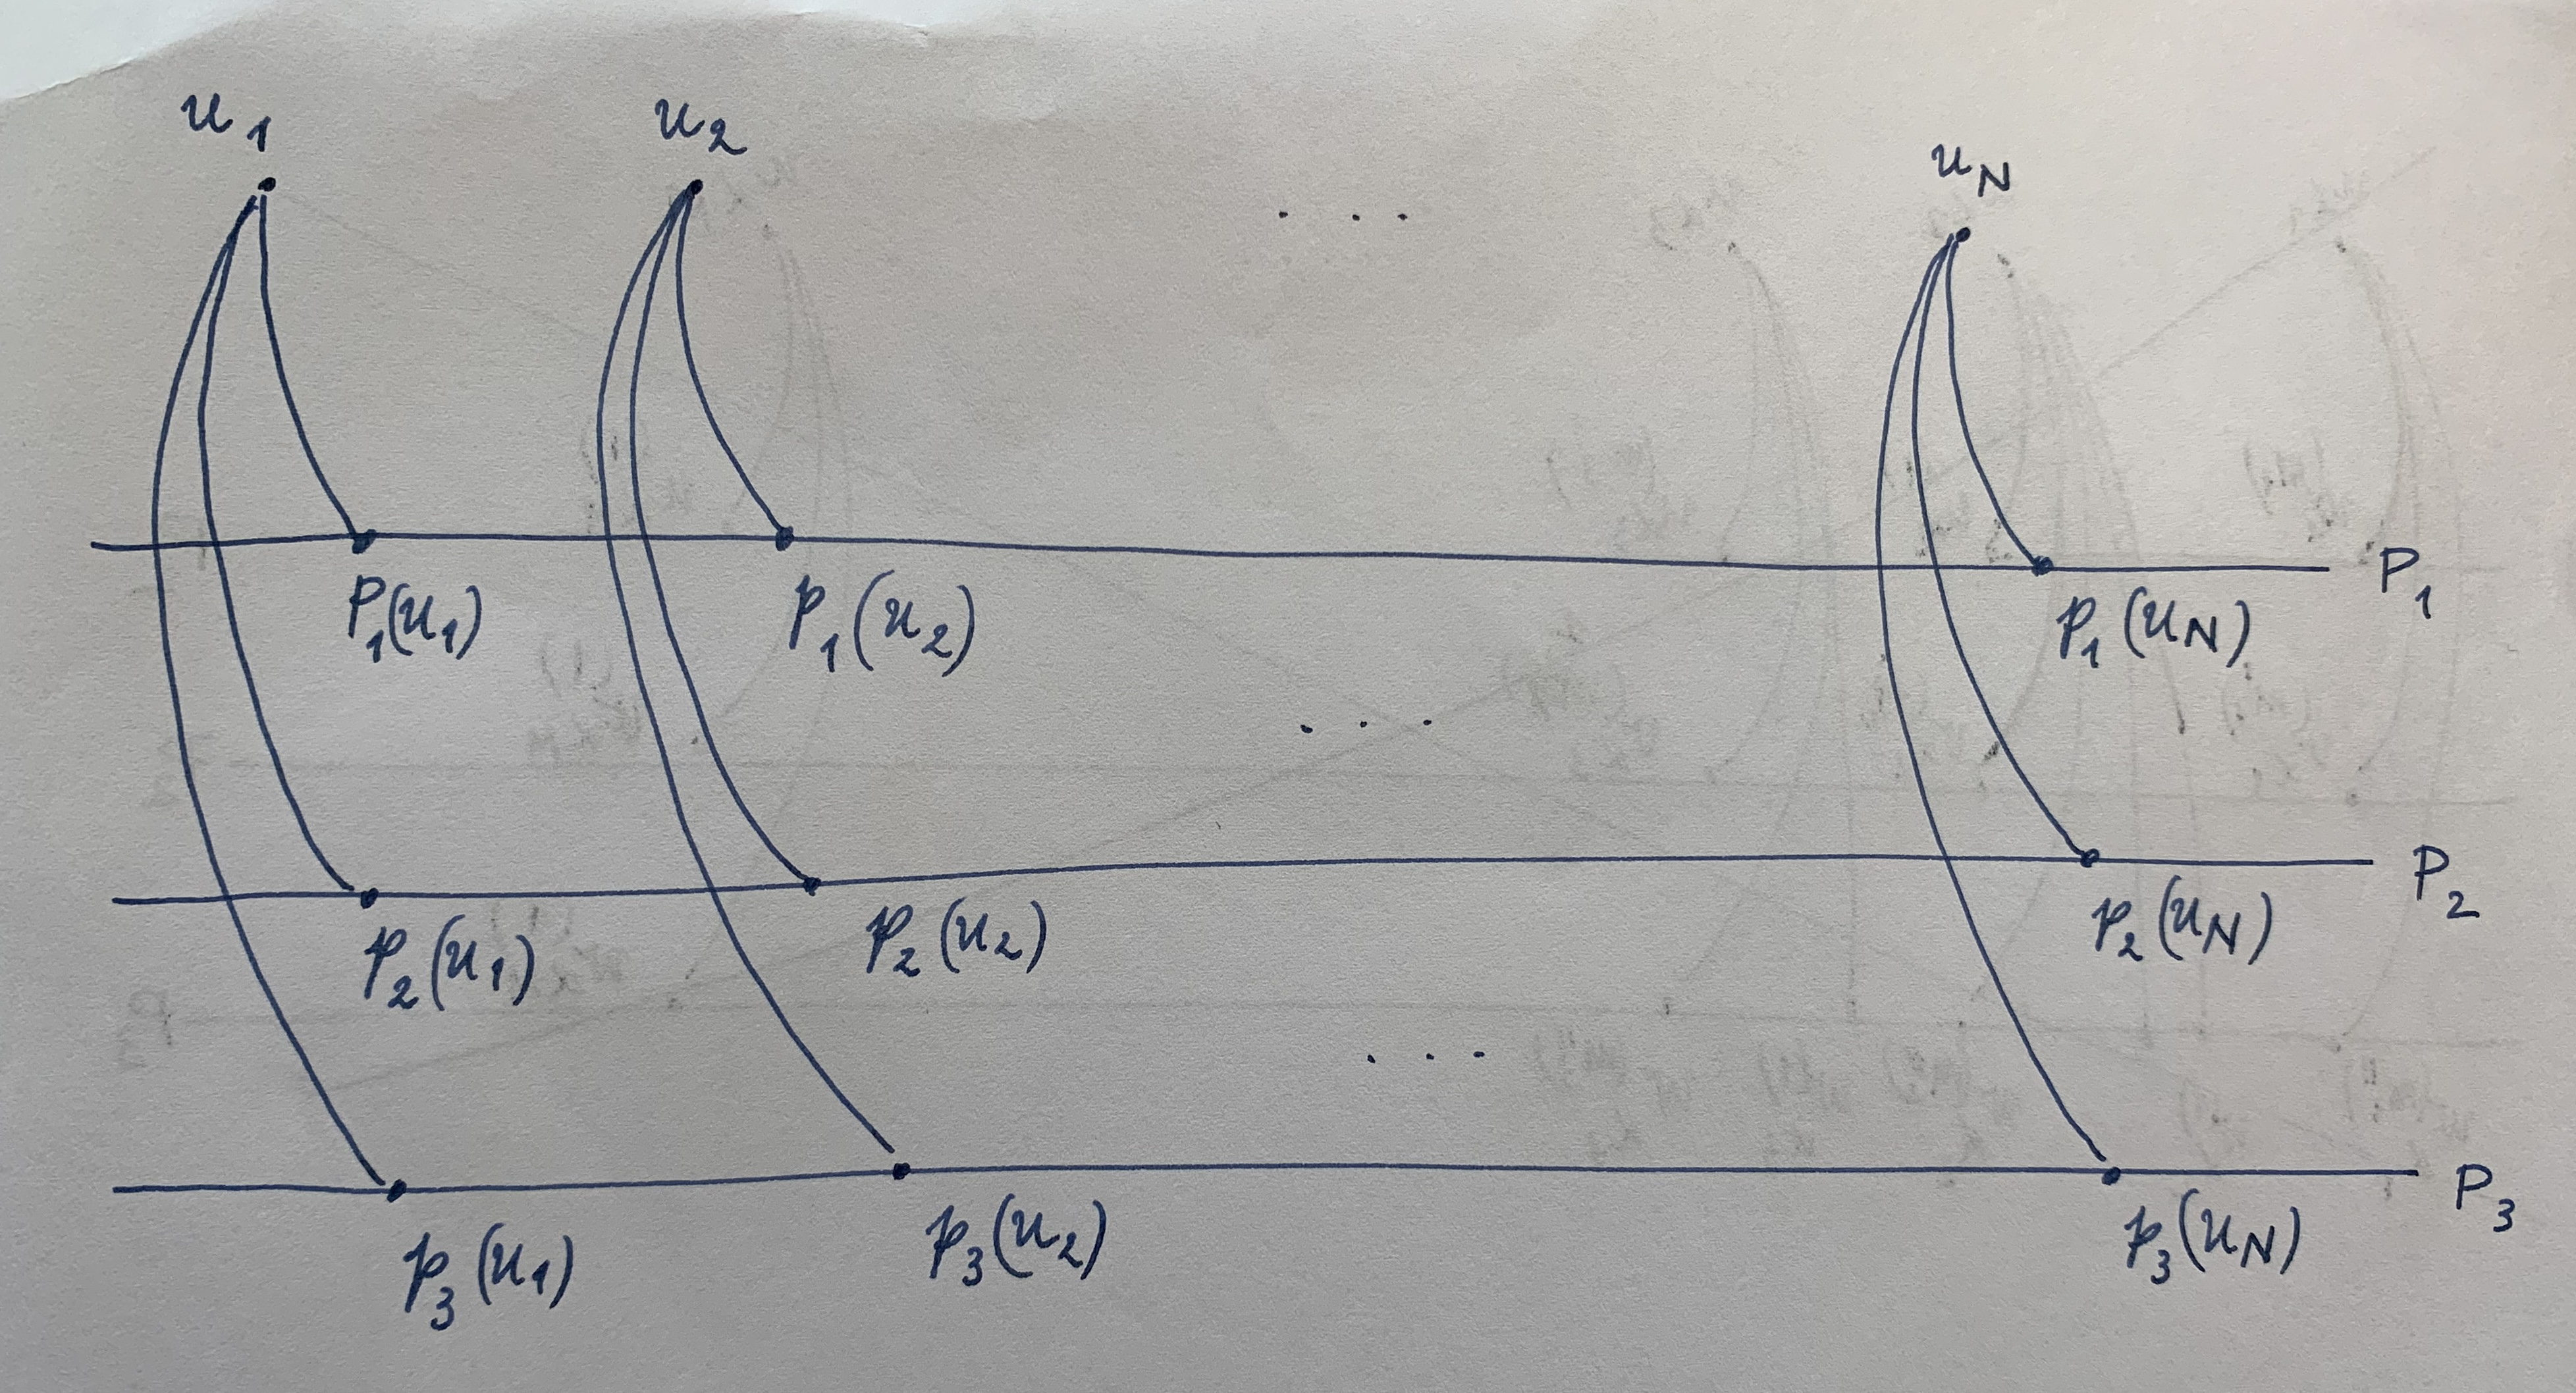
\includegraphics[width=0.75\linewidth]{figures/Erdos.jpg}
            \caption{Graph $G$ where the function $p_{j}$ 
            is increasing for all $j \in \left\{1, 2, 3\right\}$.}
            \label{fig:Erdos}
        \end{figure}


        We now inductively construct 
        a family $\left(u_{i_{j}}\right)_{j=1}^{M}$ 
        for $M$ to be determined later on,
        but only depending on $k$ with
        the following property.
        For any $u_{i} \in A$,
        denote $p_1\left(u_{i}\right) = 
        u_{i}^{\left(1\right)} \preceq_1 \cdots
        \preceq_1 u_{i}^{\left(k_{i}\right)}$
        the neighbours of $u_{i}$ in $P_1$.
        Then we have $\Gamma$:
        ``For all $1 \leq l \leq M$,
        there exists $m_{l}$ with
        $u_{i_{l}}^{\left(i\right)} \preceq_1 
        u_{i_{l}}^{\left(m_{l}\right)} \preceq_1
        u_{i_{l}}^{\left(k_{i_{l}}\right)}$ 
        such that for all $1 \leq m \leq m_{l}$,
        and all $p < l$,
        $u_{i_{p}}^{\left(m_{p}\right)}
        \preceq_1 u_{i_{l}}^{\left(m\right)}$ 
        and for all $m > m_{l}$, 
        $u_{i_{M}}^{\left(1\right)}
        \preceq_1 u_{i_{l}}^{\left(m\right)}$''.
        For an illustration refer to Figure \ref{fig:nest}.
        \begin{figure}[ht]
            \centering
            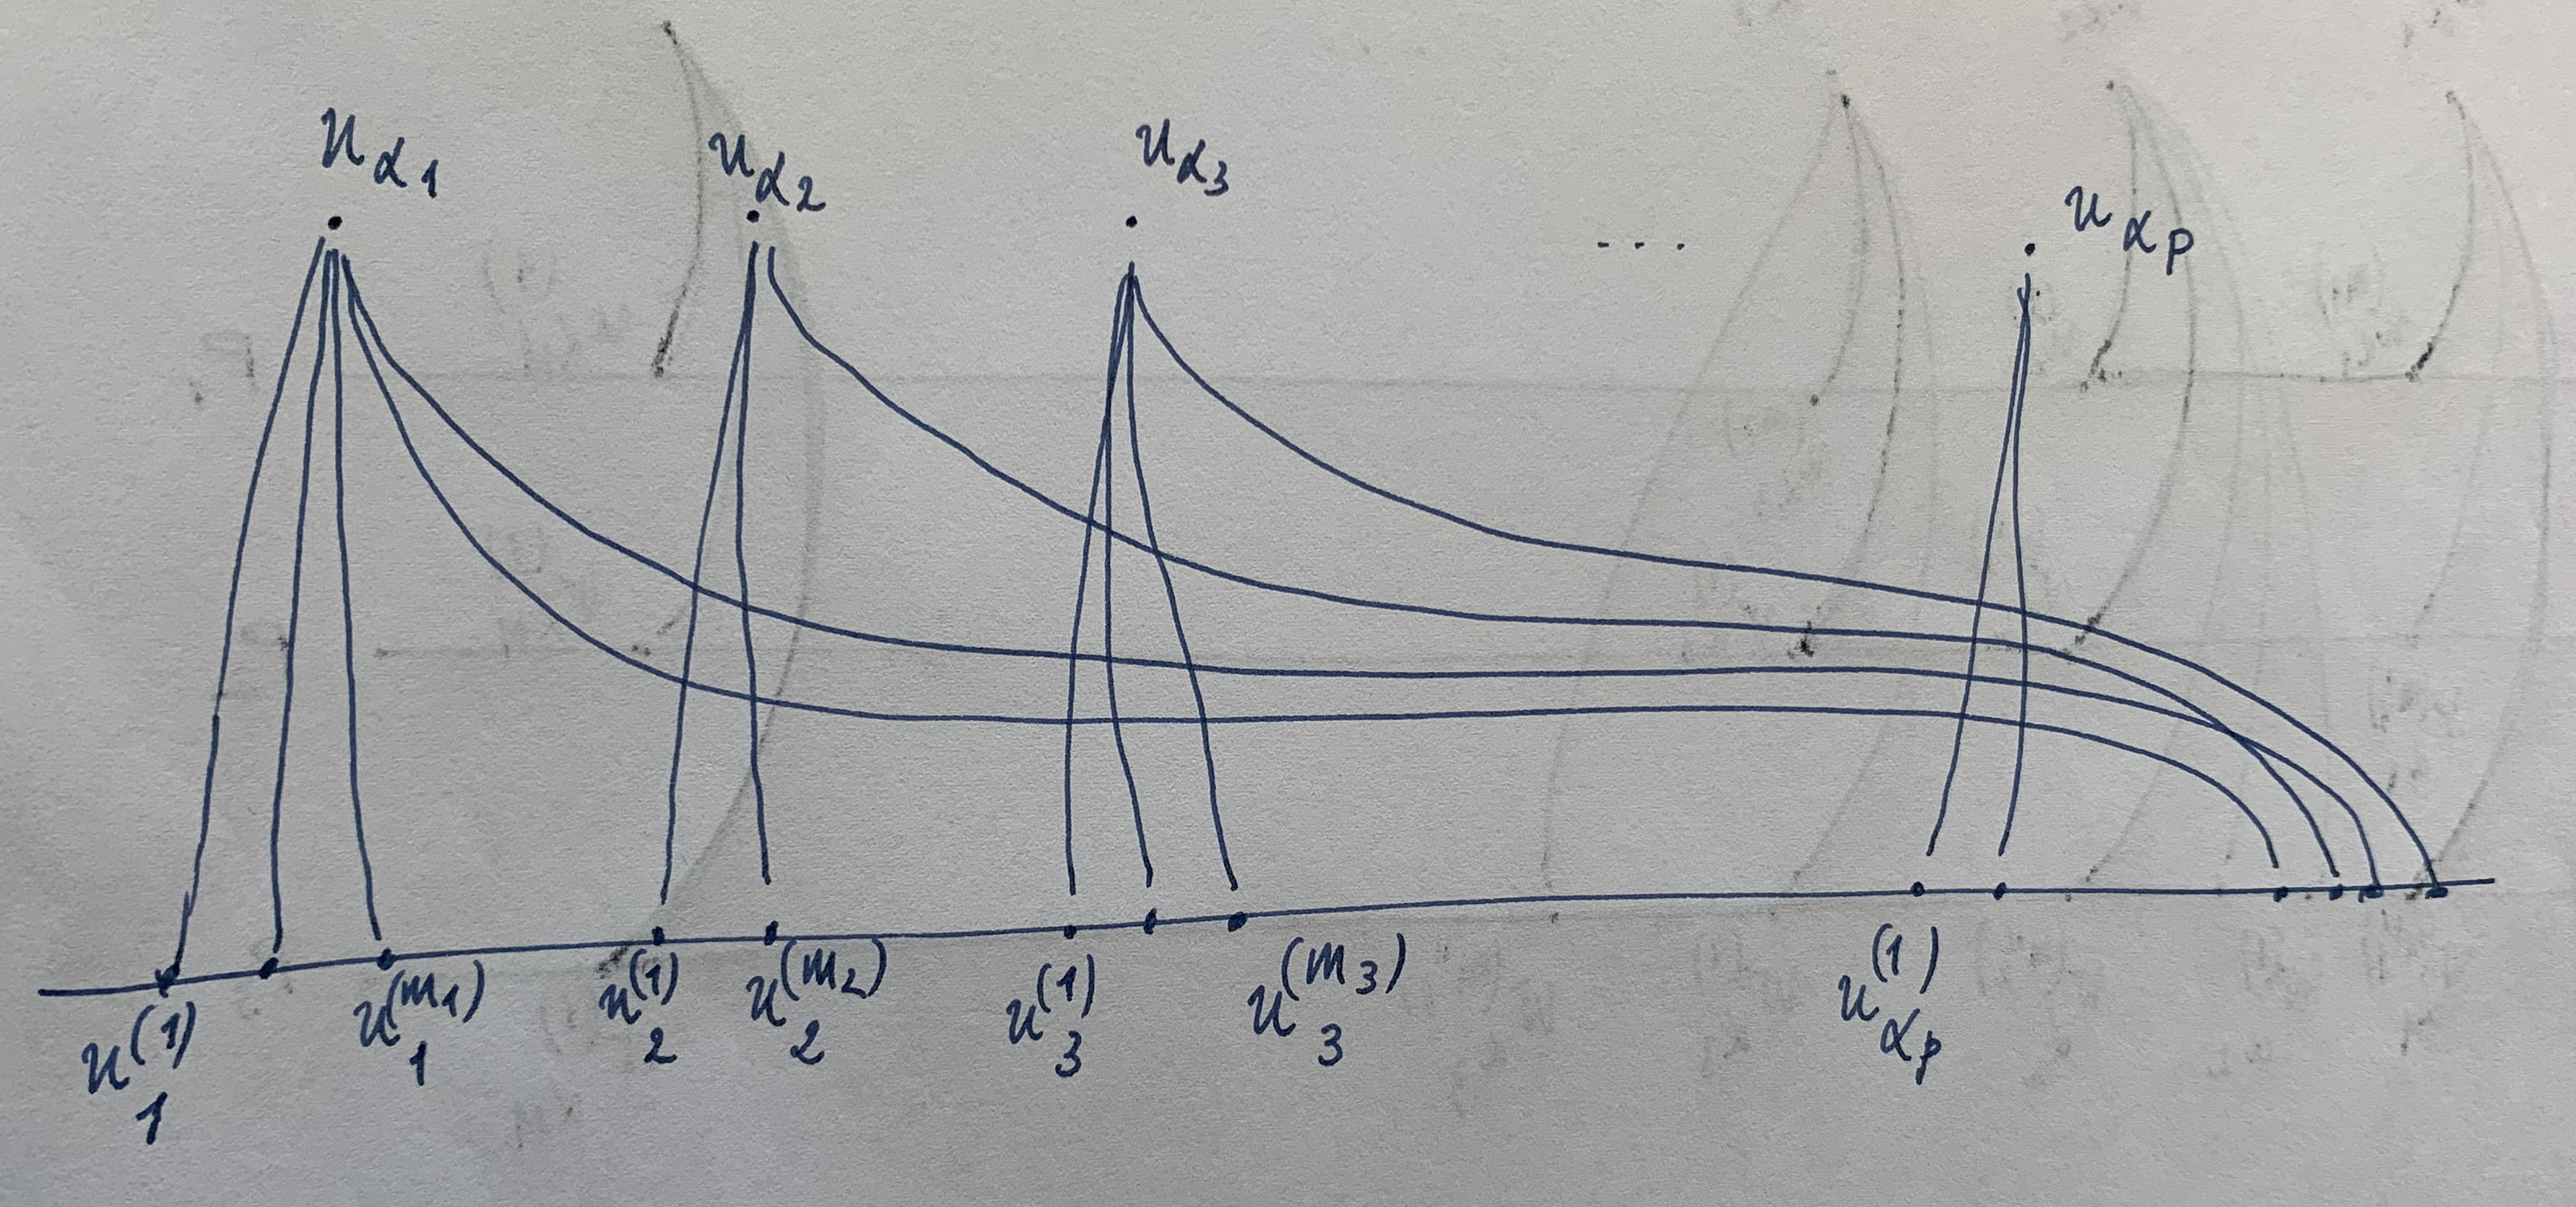
\includegraphics[width=0.75\linewidth]{figures/nest.jpg}
            \caption{Outcome of the construction satisfying $\Gamma$.}
            \label{fig:nest}
        \end{figure}

        \begin{itemize}
            \item \textbf{Base case}.
                Let $q_0 \defeq 0$ and let 
                $A \eqdef S^{\left(0\right)}_{q_0}$.
                Let also
                $i_1 \defeq 1$. For any
                $1 \leq q \leq k_1 - 1$,
                let $S^{\left(1\right)}_{q}
                \defeq \left\{u_{i}
                \middle| u_1^{\left(q\right)} \preceq_1
                u_{i}^{\left(1\right)} \preceq_1 
                u_1^{\left(q+1\right)}\right\}$
                and let
                $S^{\left(1\right)}_{k_1} \defeq
                \left\{u_{i} \middle|
                u_1^{\left(k_1\right)} \preceq_1
                u_{i}^{1}\right\}$.
                Notice that the
                $S^{\left(1\right)}_{q}$s
                form a partition of $S^{\left(0\right)}_{q_0}$ ($= A$).
                So, for any constant  $N^{\left(1\right)} \in \mathbb{N}$
                only depending on $k$, we can ask $N$
                to be big enough so that for some
                $1 \leq q_1 \leq k_1$, we have
                $\left|S_{q_1}^{\left(1\right)}\right|
                \geq N^{\left(1\right)}$.
                Let $G^{\left(1\right)}$ be the subgraph
                of $G$ induced by $S^{\left(1\right)}_{q_{1}}$,
                $P_1$, $P_2$, $P_3$.
            \item \textbf{Induction step}.
                Suppose that the set $S^{\left(l\right)}_{q_{l}} \subseteq A$
                and the indices $i_{1}, \ldots, i_{l}$
                have been set. Define the graph $G^{\left(l\right)}$
                analogously as in the base case.
                If $l \leq M-2$, 
                we can use the same
                argument as in the base case by looking
                at $G^{\left(l\right)}$
                and choosing $u_{i_{l+1}}$ 
                to be the vertex in $S^{\left(l\right)}_{q_{l}}$ 
                such that $u_{i}^{\left(1\right)} \preceq_1 u_{j}^{\left(1\right)}$,
                for all $u_{j} \in S^{\left(l\right)}_{q_{l}}$.
                We then find
                $S^{\left(l+1\right)}_{q_{l + 1}} \subseteq 
                S^{\left(l\right)}_{q_{l}}$ with
                $\left|S^{\left(l+1\right)}_{q_{l+1}}\right|
                \geq N^{\left(l+1\right)}$ for
                some $N^{\left(l+1\right)} \in \mathbb{N}$ 
                only depending on $k$.
                If $l = M-1$, then any choice of $u_{i_{M}}$
                out of the vertices in $S^{\left(M-1\right)}_{q_{M-1}}$ 
                will have the desired properties.
        \end{itemize}
        It is clear by the above construction and
        in particular by the definition 
        of the sets $S_{q_{l}}^{\left(l\right)}$ and
        by the fact that $p_1$ 
        is increasing that $\Gamma$ is satisfied.

        Since $M$ is arbitrarily large and depends only
        on $k$, we can repeat this same argument
        relatively to $P_2$ by taking only
        the family $\left\{u_{i_{j}}\right\}_{j = 1}^{M}$ 
        into consideration.
        We reiterate this for $P_3$.
        We finally get a family
        $\left\{u_{\alpha_{j}}\right\}_{j = 1}^{P}$
        so that $\Gamma$ holds
        for $P_1$ and analogous versions
        of $\Gamma$ hold for $P_2$ and
        $P_3$.

        A word on notation. Let $u_{i} \in \left\{u_{\alpha_{j}}\right\}
        _{j=1}^{P}$, denote by
        $p_2\left(u_{i}\right) = v_{i}^{\left(1\right)}
        \preceq_2 \cdots \preceq_2 v_{i}^{\left(k_{i}'\right)}$ 
        (resp. $p_3\left(u_{i}\right) = 
        w_{i}^{\left(1\right)} \preceq_3
        \cdots \preceq_3 w_{i}^{\left(k_{i}'\right)}$)
        the neighbours of $u_{i}$ in $P_2$ 
        (resp. $P_3$). 
        The index analogous to $m_{l}$
        in the construction relative to the
        path $P_2$ (resp. $P_3$) is denoted by
        $m_{l}'$ (resp. $m_{l}''$) for all
        $1 \leq l \leq P$.

        Now, consider the $k'$-chord induced by 
        the following cycle:
        \begin{gather*}
            \mathcal{K} = \left(u_{\alpha_1}, u_{\alpha_1}^{\left(m_1\right)},
            \ldots,
            u_{\alpha_2}^{\left(1\right)},
            u_{\alpha_2},
            v_{\alpha_2}^{\left(m_2'\right)},
            \ldots,
            v_{\alpha_3}^{\left(1\right)},
            u_{\alpha_3}, \ldots,
            u_{\alpha_{P}},
            w_{\alpha_{P}}^{\left(1\right)},
            \ldots,
            w_{\alpha_1}^{\left(m_1''\right)},
            u_{\alpha_1}\right).
        \end{gather*}
        Refer to Figure \ref{fig:kchord} for
        an illustration of the construction of $\mathcal{K}$.
        \begin{figure}[ht]
            \centering
            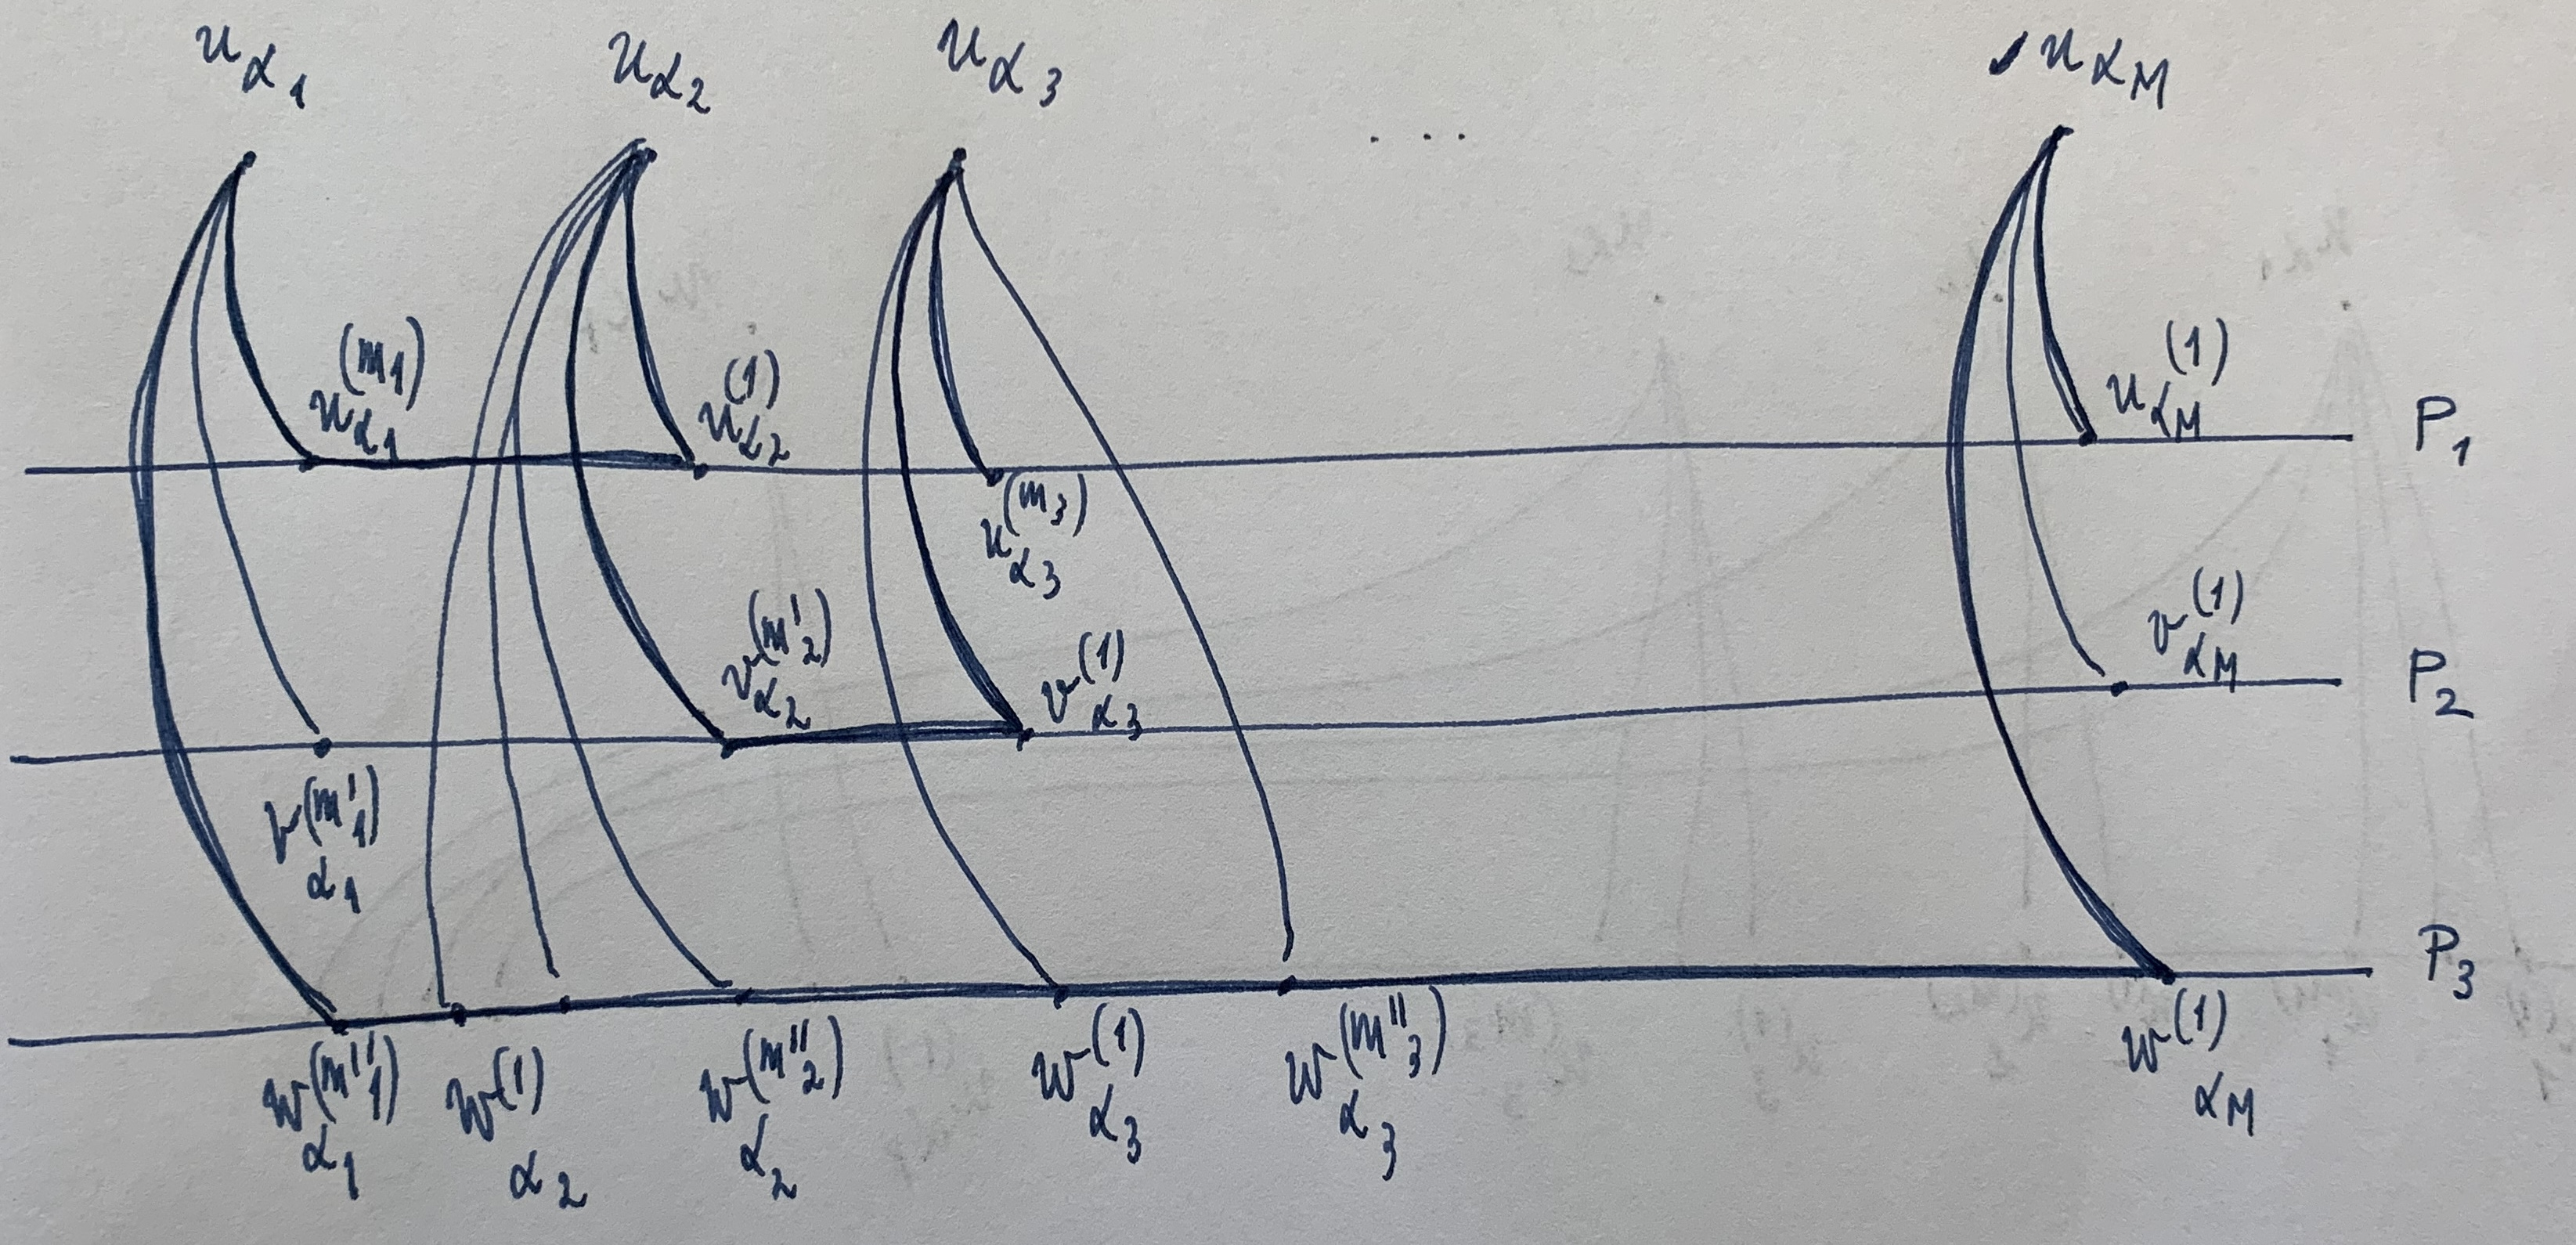
\includegraphics[width=0.75\linewidth]{figures/kchord.jpg}
            \caption{Construction of the $k'$-chord $\mathcal{K}$.}
            \label{fig:kchord}
        \end{figure}

        Since the $P_{j}$s are induced paths,
        they are chordless and there are no
        edges connecting them. We can also
        assume without loss of generality
        that for any $1 \leq i \leq P-1$,
        we have $u_{i}^{\left(1\right)} \not \sim 
        u_{i+1}^{\left(1\right)}$,
        $v_{i}^{\left(1\right)} \not \sim
        v_{i+1}^{\left(1\right)}$,
        $w_{i}^{\left(1\right)} \not \sim
        w_{i+1}^{\left(1\right)}$.
        If not, we can carry the same
        construction as before to obtain,
        instead of $\left\{u_{\alpha_{i}}\right\}_{i=1}^{P}$,
        the family $\left\{u_{\alpha_{i}}\right\}_{i=1}^{2P}$ 
        and considering in the construction of
        $\mathcal{K}$ only the subfamily
        $\left\{u_{\alpha_{2i + 1}}\right\}_{i=0}^{P-1}$.

        Thus, by construction, the only chords of
        $\mathcal{K}$ are those of the form
        $\left\{v_{\alpha_{i}}, w_{\alpha_{i}}^{\left(m\right)}\right\}$ 
        for $2 \leq i \leq P-1$ and
        $1 \leq m \leq m_{i}''$.
        Therefore, $\mathcal{K}$ has at
        least $P-2$ chords. Setting
        $P \defeq k + 2$, we get that
        $\mathcal{K}$ has at least $k$ chords.

        By the construction carried out
        trough this proof, we have that
        $w_{\alpha_{i}}^{\left(m_{i}''\right)}
        \preceq_3 w_{\alpha_{i + 1}}^{\left(1\right)}$
        for all $1 \leq i \leq P$.
        Therefore, $\mathcal{K}$ is outerplanar.
        We use Lemma \ref{lemma:outerplanar}
        to get an induced $k$-chord in $G$.

        Notice that all the constants involved in the
        above construction only depend on $P$,
        which, in turn, only depends on $k$.
        We thus set $f\left(k, 1\right) \defeq \mathbb{N}$,
        which concludes the proof.
    \end{proof}
    
    \printbibliography

\end{document}



